\documentclass[11pt]{article}
%%
%% Package includes to provide the basic style
%%
\usepackage[top=3.5cm, bottom=3.5cm, left=2.5cm, right=2.5cm]{geometry}
\usepackage{hyperref}
\usepackage{pdfpages}
\usepackage{algorithm2e}
\usepackage[authoryear]{natbib}
\bibliographystyle{plainnat}
\usepackage{appendix}
\usepackage{pgfplotstable}
\usepackage[font={color=darkgray,footnotesize, sf, it}]{caption}
\usepackage{amsmath}
\usepackage{helvet}
\usepackage{wrapfig}
\usepackage{multicol}
\usepackage[eulergreek]{sansmath}
\usepackage{listings}
\usepackage{setspace}
\usepackage{graphicx}
\usepackage{longtable}
\usepackage{minted}
\usepackage{relsize}
\linespread{1.2}
\lstset { %
    language=C++,
    backgroundcolor=\color{black!5}, % set backgroundcolor
    basicstyle=\ttfamily\footnotesize,% basic font setting
}
\usepackage{bchart}
\usepackage{booktabs}
\usepackage{xcolor}

\definecolor{skyblue}{RGB}{203,240,255}
\definecolor{forestgreen}{RGB}{0,96,50}
\definecolor{indigo}{RGB}{4,87,239}
\definecolor{darkindigo}{RGB}{1,40,112}
\definecolor{darkpurple}{RGB}{32,14,104}
\definecolor{apple}{RGB}{0,158,13}
\definecolor{bad}{RGB}{239,55,55}
\definecolor{badtoavg}{RGB}{247,128,98}
\definecolor{avg}{RGB}{255,218,117}
\definecolor{avgtogood}{RGB}{190,247,140}
\definecolor{good}{RGB}{102,226,102}

\setlength{\parindent}{0em}
\setlength{\parskip}{1em}
\setlength\parindent{0pt}

\usepackage{titling}
\usepackage{titlesec}
\pretitle{\Huge\bfseries}
\posttitle{\par}

\titlespacing\section{0pt}{12pt plus 4pt minus 2pt}{0pt plus 2pt minus 2pt}
\titlespacing\subsection{0pt}{12pt plus 4pt minus 2pt}{0pt plus 2pt minus 2pt}
\titlespacing\subsubsection{0pt}{12pt plus 4pt minus 2pt}{0pt plus 2pt minus 2pt}

\usepackage[english]{babel}
\usepackage[utf8]{inputenc}
\usepackage{fancyhdr}
 
\pagestyle{fancy}
\fancyhf{}
\rhead{cjd47}
\lhead{CM30141: \textit{Theory of Human-Computer Interaction}}
\cfoot{\thepage} 
\renewcommand{\headrulewidth}{1pt}
\renewcommand{\footrulewidth}{1pt}

\newcommand\wordcount[1]{
\vfill
\textit{Word count: {#1} words (not inc. Citations, Figures or References)}}

\newcommand\essaytitle[1]{
\begin{LARGE}
\textbf{{#1}} \\
\end{LARGE}}

\newcommand\sectiontitle[1]{
\begin{large}
\textbf{{#1}} \medskip \\ 
\end{large}}

%%
%% END OF DEFINITIONS
%%

\begin{document}
\essaytitle{Critical Review: Improving the Efficacy of Games for Change Using Personalization Models}

\sectiontitle{Introduction}
Persuasion is the act of influencing or reinforcing certain attitudes and behaviours \citep{khaled2008} and use of technology for this purpose to benefit users or the wider community is a long-term area of research \citep{fogg2002}. This review summarises and critical analyses \citet{orji2017} whose paper explores the use of personalisation models as a persuasive device for improving the efficacy of games designed to change user behaviour, to determine future work in this domain of Persuasive Technology.

\sectiontitle{Summary of Contributions}
\citet{orji2017} discuss the rising prominence of \textit{games for change}\footnote{An annual festival exists for workshops and design classes on games for change: \url{www.gamesforchange.org}} designed for purposes other than entertainment, to educate players about topics in a way that influences their behaviour \citep{busch2015}. Many such games are designed with a problematic ``\textit{one size fits all}'' philosophy - the game design (i.e. its adopted persuasive \textit{strategies}) are not tailored to the \textit{type} of player. \citet{orji2017} therefore seek to answer two main research questions to understand if the efficacy of certain strategies in existing games \citep{peng2009,kaipainen2012} can be maximised by catering to the \textit{type} of player. Firstly, whether tailoring games for change to a specific player type increases their persuasiveness. Secondly, if beneficial effects of tailoring are indeed observed, whether these are mediated by an improved playing experience. By answering these, results may inform decisions of games designers as to which persuasive strategies they adopt to maximise efficacy in certain player types. 

Treating user groups in a monolithic way is generally considered dangerous, especially in the domain of games for health \citep{berkovsky2010}.  To justify the need for investigating tailoring, the authors review persuasive strategies adopted in a range of existing domains of games for change: healthy eating \citep{kaipainen2012, orji2013b}, physical activity \citep{fujiki2008} and disease management \citep{brownson2007}. By their own admission, this list is not exhaustive which gives great scope for future research in other domains. There is clearly little work on isolating the persuasive strategies employed in these games to study their effects on specific types of gamer which makes a strong case for their research. Further, from looking at these papers describing existing games, little to no explanation is given on the behavioural theories underpinning the choice of strategies. 

To evaluate their research questions, \citeauthor{orji2017} implemented two versions of a custom model-driven online game called \textit{Junk Food Aliens} (Figure \ref{fig:orji2017-junk-food-aliens}) which targets the domain of healthy eating - players control an avatar and search for fruits and vegetables to save the planet from an invasion of junk foods. The reward-based version (JFA-R) adopted persuasive strategies such as achievement badges (Figure \ref{fig:orji2017-junk-food-aliens-reward}) whereas the competition-based version (JFA-C) adopted comparative strategies such as leaderboards displaying fictional scores of opponents (Figure \ref{fig:orji2017-junk-food-aliens-competition}). 

\begin{figure}[H]
\centering
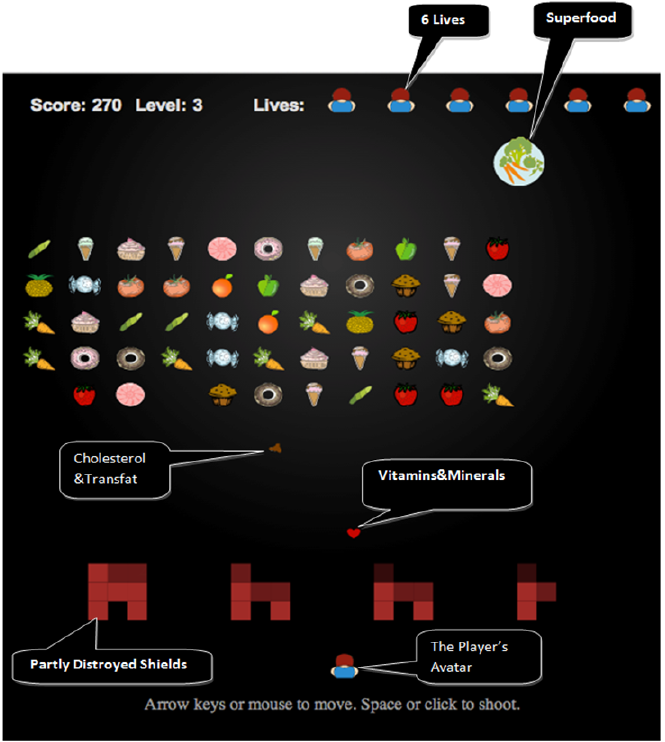
\includegraphics[width=0.4\textwidth]{img/orji2017-junk-food-aliens.png} 
\caption{``Junk Food Aliens'' (JFA): A persuasive game designed to change gamer behaviour towards healthy eating.}\label{fig:orji2017-junk-food-aliens}
\end{figure}

\begin{figure}[H]
\minipage{0.5\textwidth}
\centering
  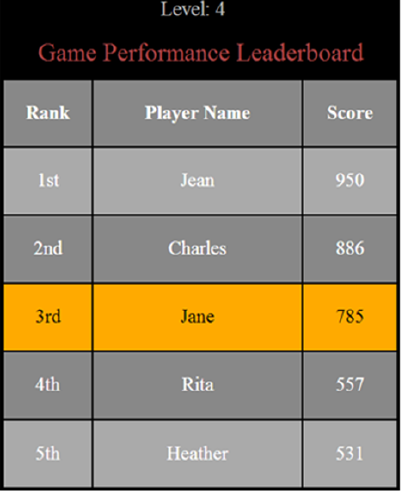
\includegraphics[height=4cm]{img/orji2017-junk-food-aliens-competition.png}
  \caption{JFA-C: Competition-based version of JFA.}\label{fig:orji2017-junk-food-aliens-competition}
\endminipage\hfill
\minipage{0.5\textwidth}%
\centering
  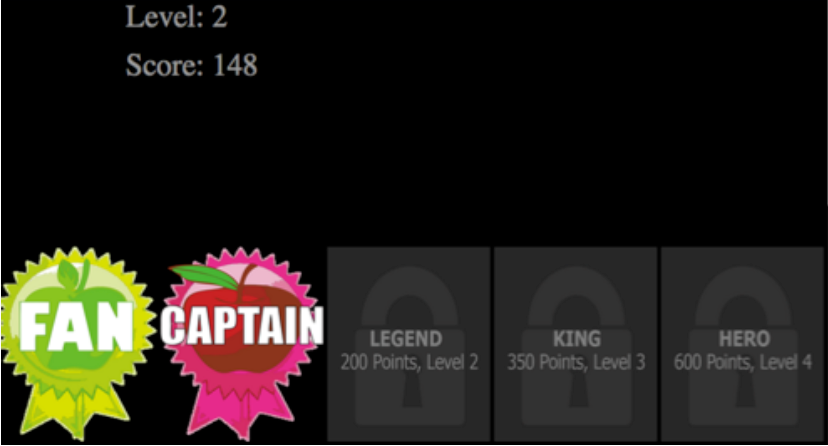
\includegraphics[height=4cm]{img/orji2017-junk-food-aliens-reward.png}
  \caption{JFA-R: Reward-based version of JFA.}\label{fig:orji2017-junk-food-aliens-reward}
\endminipage
\end{figure}

Main contributions of \citet{orji2017} are fourfold. First, it is important to tailor games for change in order to observe any efficacy (the main experiment demonstrates this by measure of change in values of precursors of behavioural change - \textit{attitude}, \textit{self-efficacy}, and \textit{intention}). Second, tailoring can be achieved by modifying the persuasive strategies adopted, rather than the mechanics of the game which minimises the costs involved in tailoring. Thirdly, the positive effect of tailoring was not mediated by an improved player experience (if not considered, this would be a potentially influential confounding factor). Finally, the adoption of a single persuasive strategy is sufficient to observe these effects - combining additional strategies is unpredictable and may be somewhat counter-productive.

\sectiontitle{Justifications for Conclusions}
The authors' initial work suggested that an effective persuasive strategy for one type of gamer could be detrimental to another by means of a lower, or negative response to motivation levels \citep{orji2013a} (Table \ref{tbl:orji2017-beta-sem}). This taxonomy forms a solid model to base the development of the JFA on, mapping independent gamer types defined by the BrainHex model \citep{nacke2014} against 8 common and pairwise distinct persuasive strategies selected by \citet{gerling2014}. Results are based on a large-scale online survey of 1108 gamers who indicated how likely each of 10 selected strategies would influence eating decisions, using a validated scale \citep{drozd2012} before completing the BrainHex questionnaire to indicate their gamer type. The data collected from this initial experiment therefore forms as valid justification for the later comparison between Achievers (motivated by Reward) and Conquerors (motivated by Competition) as they are almost polar opposites in their responses to these strategies. Use of a custom model over a more general model such as Fogg's Behavioural Model (FBM) \citep{fogg2002} increases its applicability to persuasive \textit{games}, instead of persuasive technology in general. This is at the cost of a need to re-analyse the chosen model for every new domain explored.

\begin{table}[H]
\centering
\caption{$\beta$ values confusion matrix: Strength of motivation of different players that result from different strategies. Positive $\beta$ values indicate that gamers of this type are motivated by the corresponding given strategy. Negative $\beta$ values indicate demotivation, whilst an empty value indicates neither motivation nor demotivation \protect\citep{orji2013a}.
}\label{tbl:orji2017-beta-sem}
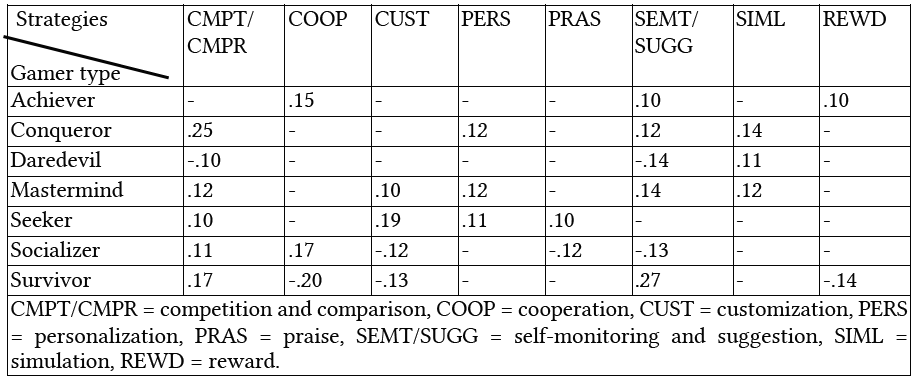
\includegraphics[width=0.75\textwidth]{img/orji2017-beta-sem.png} 
\end{table}

To empirically evaluate this model, for the rest of the paper the authors focus on games for healthy eating and restrict considerations on the effects two persuasive strategies (Competition and Reward) on two types of gamers (Achiever and Conqueror). Whilst somewhat limiting in scope, this approach allowed direct comparison between types of gamers shown empirically to be significantly-distinct in their response to these strategies \citep{orji2013a}. Furthermore, these strategies are common to existing games \citep{bell2006} and these player types are equally as dominant \citep{bartle1996}. 

Participants of the main experiment were recruited online via Amazon’s Mechanical Turk (AMT) using the guidance of \citet{mason2012}. The authors recognise this trade-off between access to a large selection pool in return for greater difficulty ensuring participant motivation or attentiveness, leading to a potential loss of generalisability in results. After two pilot studies ($N=40, N=4$) verified experimental and instrumental validity, a large-scale randomized controlled online study of 272 valid participants (117 female, 155 male - 50\% Achievers and 50\% Conquerors, all game-players) investigated the effects of tailoring and contra-tailoring on these two types of gamer in a between-subjects design. In this sense, half of Achievers played JFA-R (tailored) and the remaining half played JFA-C (contra-tailored), and vice versa for the Conquerors (tailored played JFA-C and contra-tailored played JFA-R). Participant selection was weakened by its focus on self-selected experienced gamers who are not the prime target audience for games for change \citep{brox2011}.

Before playing, participants completed a BrainHex survey \citep{nacke2014}, demographic survey and responded to 3 scales to measure their baseline attitude, intention and self-efficacy towards healthy eating based on \citet{ajzen2002}. Once gameplay began, interruptions were displayed after each minute to show rewards or the leaderboard in JFA-R and JFA-C respectively. After participants finished playing their assigned version of JFA for 20 minutes, they responded to the same 3 scales to measure their post-task attitude, intention and self-efficacy towards healthy eating. Finally, they also assessed their experience (enjoyment, effort, competence and tension) \citep{ryan2006}. Results showed tailoring the game to a specific gamer type increased effectiveness (measured by positive changes in attitudes, intentions and self-efficacy towards healthy eating) while contra-tailoring did not (Figure \ref{fig:orji2017-tailoring-results}).

\begin{figure}[H]
\centering
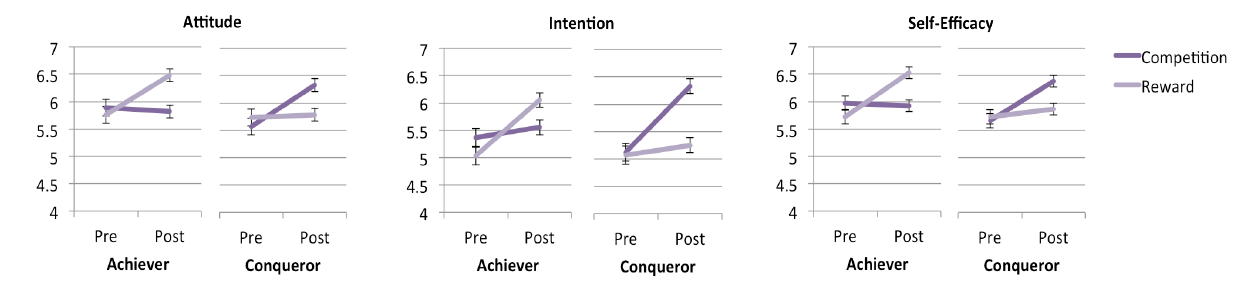
\includegraphics[width=\textwidth]{img/orji2017-tailoring-results.png} 
\caption{Mean values $\pm$ SE for Attitude, Intention, and Self-Efficacy by Gamer type (Achiever, Conqueror) and Game version (Competition, Reward).}\label{fig:orji2017-tailoring-results}
\end{figure}

Parallel mediated regressions \citep{hayes2013} showed the positive effects of tailoring were not mediated by improved player experience which provides strong support in favour of tailoring games to player type (Figure \ref{fig:orji2017-tailoring-mediation-results}). 

\begin{figure}[H]
\centering
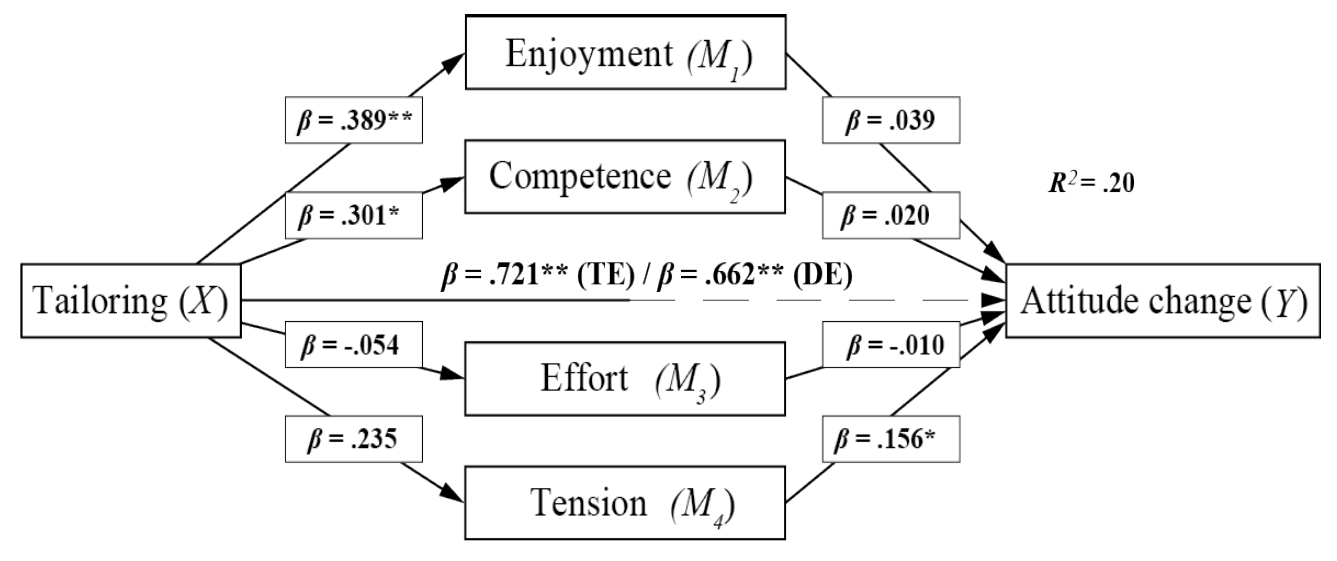
\includegraphics[width=0.75\textwidth]{img/orji2017-tailoring-mediation-results.png} 
\caption{Parallel mediation model of tailoring on attitude change with play experience as mediator.}\label{fig:orji2017-tailoring-mediation-results}
\end{figure}

There is a respectable amount of evidence to support the authors' claims. The number and representativeness of the participant sample has been carefully considered, with the limitations of using AMT discussed.

\sectiontitle{Limitations and Suggested Further Work}
Whilst the findings of the main experiment are convincing, well designed and validated with a good report on parametric data gathered, there are a series of limitations and unanswered questions that must be considered.

\citeauthor{orji2017} appreciate that scoping their main experiment to focus only on Achievers and Conquerors under Reward and Competition strategies respectively should encourage future research on different combinations of strategies and different gamer types. Their current research limits itself to the measure of change in attitude, intention, and self-efficacy toward healthy eating which immediately prompts questions about its effects on \textit{tangible} changes in behaviour, rather than effects on \textit{mediators} or \textit{precursors} of behaviour change. Also, although purely illustrative, the domain choice of healthy eating should not limit investigations - by applying their model to other domains such as disease management and physical activity, it will be possible to decipher whether the effects of the persuasive strategy employed are domain-dependent. That said, the custom model cannot be immediately generalised to domains other than healthy eating without careful further investigation.

Ideally, participant recruitment should be intrinsically motivated rather than via AMT where not all participants may be psychologically engaged in tasks affecting generalisability of results. It would also be novel to explore the adoption of a single persuasive strategy compared with use of multiple in a given game, to observe whether compounding effects are positive or negative on efficacy of behaviour change. Now that we are aware that player experience does not mediate the observed benefits, it would be wise to also consider whether \textit{game performance} as a potential mediating factor - players who perform better in the game under a given strategy may experience more positive feeling towards the tailored game which could influence the observed results. The current approach is also somewhat static in nature once participants are assigned to a given gamer type. Answers to the BrainHex questionnaire are what determines a player's type. Instead, it might be interesting to explore the avenue of determining a player's type in a more dynamic sense, perhaps during actual gameplay based on activity or game events. Future research should also consider effects on non-gamers seeing as many existing persuasive games cater for this group - e.g. the elderly population \citep{deoliveira2010}.

Another novel suggestion to build on these findings is to experiment with existing gamification applications for physical exercise such as Apple Watch and Nike+ GPS, instead of focusing purely on games for change. By expanding into this area, this might require re-evaluation of the strategies originally selected by \citet{gerling2014}.

\sectiontitle{Conclusion}
\citet{orji2017} make a convincing case for personalising persuasive strategies employed in future games for change in order to observe effective change in behaviour. Whilst there are limitations to their work, it lays strong foundations for future work investigating tailoring games for change in other domains. Findings have potentially wider consequences in Persuasive Technology - with recommendations on how to tailor to specific groups of users whilst minimising the efforts and costs involved in doing so, designers of these technologies could better-understand the considerations needed when matching a persuasive strategy to their specific user group.

\wordcount{1646}

\newpage
\small
\bibliography{bib1}
\normalsize
\end{document}